\section{Databases}
\label{sec:databases}

The Mu2e database structure comprises several databases containing the metadata required to collect, store, process, and analyze data. An overview of information flow through Mu2e databases is shown in Figure~\ref{fig:db}. The subset of metadata needed to understand the data collected by the Mu2e detector is often referred to as condition data (e.g., detector alignment parameters or calibration constants). These data are indexed by (fraction of) runs, grouped into intervals of validity. Conditions data sampled at a lower frequency will be interpolated to match the physics requirements of the experiment. While conditions metadata will generally be stored in appropriate databases, they could be inserted in the raw detector data stream in some instances. APIs providing access to condition metadata independent of the underlying technical details will be provided to users. 

\begin{figure}[htb]
\begin{center}
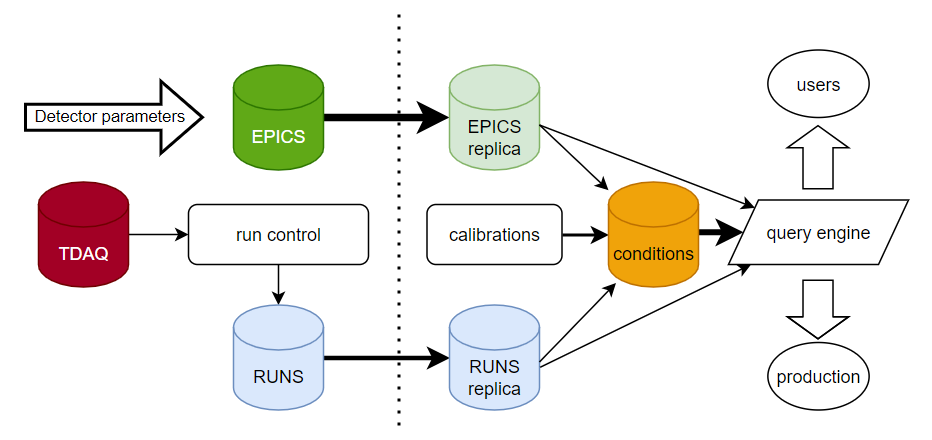
\includegraphics[width=0.8\linewidth]{figures/db.png}
\caption{An overview of information flow through Mu2e databases.}
\label{fig:db}
\end{center}
\end{figure}

Reliable access to metadata over the full lifetime of the experiment is a crucial requirement of the database system. To mitigate the risk that the underlying technology becomes obsolete during this period, Mu2e is following the general FNAL strategy of adopting open-source and widely supported products. The Mu2e DAQ system is based on MongoDB technology, while all other databases are using the PostgreSQL database management system. These databases are supported by the database group of the FNAL IT division, providing the software, the platform, and the servers (except the DAQ MongoDB database, hosted on the DAQ server to ensure continued access in case of network outage). All offline database accounts are authenticated by kerberos principles and are created by the database support group via a service desk ticket. The support group also provides a streaming service for copying from the online to the offline instance. The Mu2e workflow assumes 8/5 support for offline database with best effort outside standard hours.

All offline database content is written via SQL commands generated by Mu2e custom tools in c++ and python. Database queries are performed through the Query Engine, a lab-supported product providing an HTTP interface for all simple, high-rate queries. Two types of queries are available: reads from the web server cache (the cache refreshed with a programmable lifetime), or directly from the database via the web server. This system can be scaled to provide conditions content to jobs distributed across large numbers of grid-based or high-performance computing (HPC) systems. The service also provides valuable real-time monitoring of system response times and timelines. In addition, (partial) database content can be dumped into a file on /cvmfs and used for subsequent reconstruction or simulation tasks. This option could be useful in cases where the network bandwidth becomes limited, for example running a very large number of simulation jobs at a high-performance computing center.  

Database development is fully integrated into the Mu2e code development workflow and performed in collaboration with sub-system experts. A core principle is to maintain an automated robust audit trail of the processing history of each file, from TDAQ to final analysis datasets. This includes recording version information for code, databases and workflow configuration, and parent-child information among files. Mu2e has already recorded this information during the various simulation campaigns and we are investigating improved implementations. Among the desired features is the ability to specify that a file must be reprocessed using the same database versions that were used in the trigger.

The list of Mu2e databases is presented in Table \ref{tab:db}, and each instance is described in more detail below. 

\begin{table}[ht!]
\begin{center}
\begin{tabular}{ |l |c | c| }
\hline
label & schema & description \\ \hline
 DAQ & lab/Mu2e & DAQ configuration \\  
 EPICS & EPICS & detector metrics \\   
 run conditions & Mu2e & run metadata \\  
 offline EPICS & Mu2e & streamed from online \\  
 offline run conditions & Mu2e & streamed from online \\  
 conditions & Mu2e & calibrations \\
 DQM & Mu2e & offline data quality \\
 good run & Mu2e & good run list \\
 luminosity & Mu2e & runs luminosity \\
 SAM & lab & file metadata \\
 MetaCat & lab & file metadata \\
 Rucio & lab & file locations \\ \hline
\end{tabular}
\end{center}
\caption{Listing of Mu2e operations databases.  All are installed and managed by lab professionals.  All are postgres except DAQ, which is MongoDB.}
\label{tab:db}
\end{table}

%\begin{itemize}
%  \item DAQ configuration (online, not streamed offline)
%  \item run conditions database (online, streamed offline)
%  \item EPICS archive database (online, streamed offline)
%  \item conditions
%  \item good run
%  \item luminosity
%\end{itemize}


%\subsection{Infrastructure} \label{database-infrastructure}
%In implementing database infrastructure, we are following lab recommendations and leveraging lab expertise and support.  The DAQ database is MongoDB, but all other databases are version 14 pr 15 postgres.  The postgres databases are all hosted by the lab database group.  This support provides the postgress software, the platform, and servers. (Online database managed by the database group, but hosted on a Mu2e DAQ server.) All accounts are authenticated by kerberos principles and are created by the database support group via a servicedesk ticket.  The support group also provides a streaming service for copying from the online to offline instance.  Currently, the stream is up-to-date within 30 min, but this can be reduced to 10 min when needed.

%Offline, all database content is written by SQL commands generated by Mu2e tools, implemented using the psql exe at the command line, or libpq in c++ or psycopg2 in python.  All reads of the offline databases are through the Query Engine lab-supported product.  This system provides an http interface for all simple, high-rate database reads and is critical for providing conditions content to grid jobs.  Access is not authenticated, but is limited to on-site, VPN or select grid sites \red{need to re-check}.  There are two types of reads provided: reads from web server cache (the cache refreshed with a programmable lifetime), or directly from the database via the web server.  The service provides valuable real-time monitoring of system response times, including timelines.

%Mu2e has been operating with these systems for several years and we expect they will meet all our needs.


\subsection{Run Conditions database} 
The DAQ database is managed by the online operations group. At the beginning of each run, the DAQ system copies all information used to configure the detector and DAQ from the MongoDB DAQ database into the online run conditions database. Each run is divided into subruns, and the system records the precise times of the subruns in both wall clock time and accelerator ticks. At the end of the run, summary information (e.g. total number of processed events or run time) is added to the record. 

The online content is periodically streamed to an offline database instance. As a new run appears, offline data reconstruction is triggered and the job configuration is retrieved from the database. A web page with interactive search for data discovery also provides information about recent runs. Finally, tools are developed to extract the trigger configuration so that it can be reproduced for simulation or performance studies. 

\subsection{EPICS database}
EPICS is a system designed to monitor, display, and alarm arbitrary quantities, such as voltages, status, and environmental conditions. This stream of monitoring data is archived in an online postgres database using standard EPICS tools and then streamed to an offline instance. Users can access content through a simple custom tool (epicsTool), available both at the command line and in c++.

Environmental conditions required for detector response reconstruction is automatically extracted from the EPICS database offline instance and re-packaged in the conditions system to ensure reproducibility.

%Some detector responses are sensitive to environmental conditions. If this information is required in reconstruction, it is automatically extracted from the EPICS database offline instance and re-packaged in the conditions system for reproducibility.

\subsection{Conditions database} 
The conditions database tracks the detector conditions (e.g., pedestals, gains, bad channels,...) and their run dependence using a custom schema. The user specifies a purpose (such as "Pass~1'', "Sim2020'', or "CaloCalibration'') together with a version number to define which "conditions set'' the reconstruction job will access. The version number has three fields: the major version, used by experts to alert the user of an important change in conditions philosophy; the minor number,  indicating changes to content; and the final number, specifying the extension listing the intervals of validity. Reconstruction jobs with the same major and minor numbers will produce identical results, as a design requirement. The schema implements a closed interval of validity (with an option to relax if needed). When a repair is needed, or new types of tables need to be added, a new minor version is created.

Each detector sub-system defines the content of the tables added to the schema. In addition, "archive'' tables may be created to store intermediate results which are not used in reconstruction, but should still be saved. The system also provides "ad-hoc'' tables for secondary needs like record-keeping. A development database is available to verify the SQL commands and compatibility with code before creating the same table in the production environment. The content and intervals of validity provided by each sub-system are grouped into a condition set. 

A user interface dubbed "Proditions" provides access to the database in the reconstruction code. This layer can perform intermediate calculations based on the database contents and reorganize the data into different data structures or subsets of table data. The run-dependence of this content is automatically tracked based on the database table run dependence. Proditions has also an onboard cache to prevent thrashing.

Other implementation features include a text table option for overriding database content for testing purposes. Should the database access be unavailable, the text option can provide the entire conditions set content. A programmable onboard cache saves tables so switching back and forth between tables does not generate new fetches. All external operations are timed to evaluate the performance. Multiple layers of verbosity are provided to help debugging. The code is designed to be thread-safe as well.

All tools needed for database upload, queries, and repair have been developed. The conditions database system has already been extensively tested, and the measured performance will greatly exceed requirements for \passone, the most time-sensitive operation.  

%A development database exists with the identical schema as the production database. When a new calibration table is proposed, it is first installed in the development database to verify the SQL commands and compatibility with code, then the same table is created in production.  Other operations can be also tested first in development.  We have not found the need for an integration database yet, but if one is needed, it will be straightforward to create.

%Each subdetector defines what tables they need and they are added to the schema. The users may create "archive'' tables to store intermediate results which are not used in reconstruction, but should still be saved.  The system also provides "ad-hoc'' tables for secondary needs, like record-keeping. In operations, the subdetector expert provides content and IoV's, and passes them to the calibration coordinator, who joins the subdetector content together into a conditions set.

%All tools needed for database upload, readback, and repair exist.  The conditions database system has been in daily use for several years.  The system has been informally load-tested, and will greatly exceed requirements for pass1, the most time-sensitive operation.  A more formal load test will be coupled to raw data upload and pass1.


\subsection{DQM database} 
Data quality information may be produced at any stage of processing.  A set of analysis modules histogram critical quantities and the histogram files are preserved.  A series of tags label the files according to source, version, time, and run. A process then converts the histograms, and other information, into a series of metrics which are inserted in the DQM database. These metrics can be displayed as a function of run number or time or extracted as CSV tables for further analysis.  A system of limits provides alarms when metrics are out of tolerance.


\subsection{Good-run database} 
The definition of "good runs" will depend on the context and might involve input from the different detector sub-systems and experts. The good-run database collects information relative to run quality (typically an int) for a given interval of validity. Users can retrieve and edit this information to create a custom selection, which is then persistent in the database. The data can be accessed either by dedicated tools or within the reconstruction software. 

%Different analysis groups may define what is usable data differently and should have the ability to define what runs they want to use for a given purpose.  What is considered good may also involve input from many sub-system and other experts. The good-run database collects input from experts, as a status (typically an int) for a given IoV.  The user of these, then can define a selection, of these reports, add information from run conditions, adjust the selection by hand, then preserve the selection in the database.  Access to the good run list is by tools, or as a filter in processing.

\subsection{Luminosity database}
The number of stopped muons must be known to properly normalize the experimental results. To this end, it may be useful to track the number of protons on the primary target and other experimental quantities (e.g. the number of protons in the tracker), possibly as frequently as every micro-bunch. This large amount of data would be preserved in a database and accessed using custom tools or within the reconstruction software.

\subsection{Data-handling databases}
The data-handling database is fully designed and managed by the lab and contains standard schema. All writes are by standard tools with standard authentication systems. All reads are via load-balanced http services designed and maintained by the lab. The SAM database is a legacy system and will be deprecated before full operations.

%The number of stopped muons is the denominator in the measurement or limit for charge lepton flavor violation, the primary goal of Mu2e.  Towards this end, it may be useful to track the number of protons on the primary target, possibly as frequently as every bunch.  We will track several quantities per proton bunch, resulting in a large dataset.  We expect this will be preserved in a database, and accessed using custom tools, as an efficiency-weighted luminosity independent, of event processing on the grid. (XXX this section is weak)
